\chapter{Markov Decision Process}

Markov Decision Processes describe a time-discrete and stochastic process that can be used to model different planning and decision-making problems. MDPs are used in all kinds of domains and multiple algorithms have been proposed to solve a particular MDP. 

\section{Definition}

A MDP is defined by:

\begin{itemize}
	\item set of states ($S$)
	\item set of actions ($A$)
	\item state-transition function $P_a(s,s')$
	\item reward-function $R_a(s,s')$
\end{itemize}
The state-transition-function $P_a(s,s')$ gives the probability of transferring to a consecutive state $s'$ when in state $s$ and applying action $a$. For a given state $s$ and action $a$ the probability is independent from former states or actions. This property is referred to as the \emph{Markov property}. The goal of optimization is a scalar value referred to as the \emph{cost} or \emph{reward} which is either minimized (in case a problem defined by costs) or maximized (for rewards). The reward/cost is a function of the current state $s$ and consecutive state $s'$ given an action: $R_a(s,s')$. 

Solving a MDP requires to find a mapping from each state to an action that maximizes reward or minimizes the costs. A mapping is referred to as the \emph{policy} and is denoted by $\pi$. A policy that achieves the highest possible reward is referred to as the \emph{optimal policy}. 

\section{Algorithms}

For finite state and action spaces algorithms based on dynamic programming are a popular choice for solving MDPs. 
The foundation for applying dynamic programming to this problem class is the definition of a recursive function that assigns a value to a state given that a specific policy $\pi$ is applied.  

\begin{equation}
V_\pi = \sum_{a} \pi(a \mid s) \sum_{s^{\prime}, r} p\left(s^{\prime}, r \mid s, a\right)\left[r+\gamma v_{\pi}\left(s^{\prime}\right)\right]
\label{valuefunction}
\end{equation}

\autoref{valuefunction} is referred to as the \emph{Bellmann equation for value functions}. $\gamma$ is the \emph{discount rate} parameter: $0\leq\gamma\leq1$ 

A common algorithm is referred to as \emph{policy iteration}. In an iterative cycle the value function of each state following a policy is first evaluated (\emph{policy evaluation}) and then the policy updated (\emph{policy improvement}). This process is depicted in \autoref{GPI}.

\begin{figure}[ht]
	\centering
	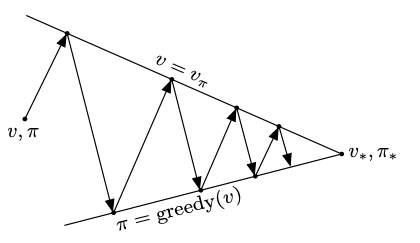
\includegraphics[width=.6\textwidth]{images/GPI2.png}
	\caption{\label{fig:bild2}Iteration between policy evaluation and policy improvement \autocite{Sutton2018}}
	\label{GPI}
\end{figure}

For both policy evaluation and policy improvement different approaches exist. When using \emph{iterative policy evaluation} and a \emph{greedy} policy update, policy iteration is guaranteed to converge to the optimal policy. Iterative policy evaluation describes the evaluation of the current policy using \autoref{valuefunction}. A greedy policy update is selecting the action with the highest expected reward according to a one-step look-ahead using the value function of a consecutive state. 
